\section{Introduction\footnote{The introduction is mostly based on \cite{ChiSym} with other references used where cited.}}
\label{sec:Introduction}
Write a bit about QGP, heavy ion collisions, phase diagram and chiral symmetry and its restoration, probes for chisym restoration here.

\subsection{The QCD Lagrangian}
To understand the effects of the strong interaction we use the theory which has been proven most succesful in this matter in the end of the last century: QCD (for a comprehensive introduction see e.g. \cite{QCDEllis}). We start from the classic Lagrangian of QCD with 3 flavours which is the unique Lagrangian which is invariant under a gauged SU(3) symmetry
\begin{equation}
\label{eqn:LQCD}
\Lag_{QCD} = \bar{\psi}_i \left( i\gamma_{\mu} D^{\mu} - m \right)_{ij} \psi_j - \frac{1}{4} G_{\mu\nu}^a G^{\mu\nu}_a
\end{equation}
where $\psi = \left( u,d,s \right)$ are the quark fields, $D^{\mu} = \partial^{\mu} -igA^{\mu}$ is the covariant derivative in the fundamental representation and $G_{\mu\nu}^a = \partial_{\mu}A_{\nu} - \partial_{\nu}A_{\mu} + g f^{abc} A_{\mu}^b A_{\nu}^c$ is the field strength of the gluon fields $A_{\mu}^a$ with the structure constants $f^{abc}$ of SU(3).
Following the usual procedure of perturbative renormalization we can calculate the $\beta$-function in QCD. At 1-loop order it is given by
\begin{equation}
\label{eqn:beta}
\beta(\alpha_S) = \mu_R^2 \frac{d\alpha_S}{d\mu_R^2} = - \left( 11 - \frac{2}{3} n_f \right) \frac{\alpha_S^2}{2\pi} + O(\alpha_S^3)  \equiv - \beta_0 \frac{\alpha_S^2}{2\pi} + O(\alpha_S^3)
\end{equation}
where $n_f$ is the number of flavours and $\beta_0$ the 1-loop $\beta$-function coefficient.
\begin{figure}[b]
	\centering
	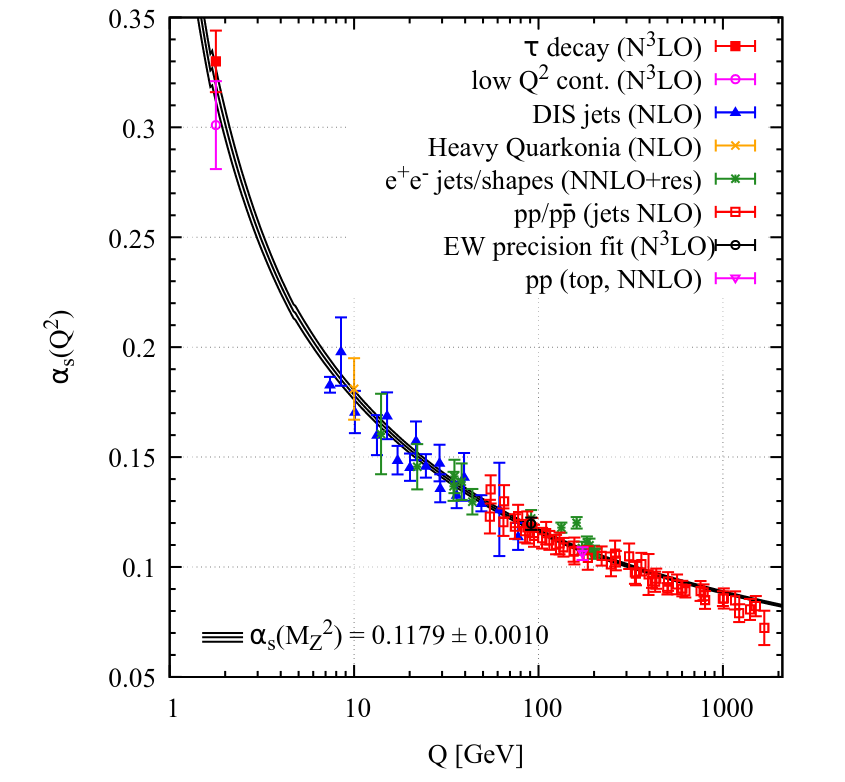
\includegraphics[width=0.55\textwidth]{Figures/alphaQCD}
	\caption{The running coupling of QCD \cite{PDG2018}. Summary of measurements of $\alpha_S$ as a function of the scale $Q$. The order in QCD perturbation theory which was used in the calculation is indicated in brackets.}
	\label{fig:alpha}
\end{figure}
Solving the differential equation in eqn. \ref{eqn:beta} in terms of the renormalized scale $\mu_R^2$ we get an expression for the running coupling in QCD. Using the 1-loop expression we get
\begin{equation}
\label{eqn:alpha}
\alpha_S(\mu) = \frac{4\pi}{\beta_0 \log\frac{\mu^2}{\Lambda^2}} 
\end{equation}
where $\Lambda$ is the QCD scale and we fixed $\alpha(\mu) \overset{\mu \rightarrow \Lambda}{\longrightarrow} \infty$. A plot of the running coupling along with the most recent measurements can be seen in fig. \ref{fig:alpha}. \\
From eqn. \ref{eqn:alpha} it is obvious that perturbation theory is not applicable at energy scales close to the fundamental scale of our theory. Unfortunately this is the regime we are interested in, so we have to think of another way to approach scales $\mu < \Lambda_{QCD}$. 
\subsection{Chiral Symmetry of QCD}
One of the ways to approach regimes where $\mu < \Lambda_{QCD}$ is to build an effective Lagrangian based on the symmetries of the fundamental Lagrangian of QCD. In this section we investigate this approach and see which implications it has for the particle spectrum of the theory. \\
We start from the Lagrangian of QCD in eqn. \ref{eqn:LQCD}. Of particular interest to us for the chiral symmetry is the quark term in the Lagrangian which can be split into two parts
\begin{equation}
\Lag_{\mathrm{quarks}} = \bar{\psi} i\gamma_{\mu} D^{\mu} \psi - m \bar{\psi} \psi \equiv \Lag + \delta\Lag
\end{equation}
The suggestive names will make sense in a second. 
Since the doublet of quark fields in $\Lag$ are contracted in an inner product the Lagrangian is invariant under an inner symmetry. In our case this is a U(2) symmetry for both chiralities, so U(2)$_L \times$ U(2)$_R$ in total. We can also think of the symmetries in terms of axial and vector currents instead of left and right handed currents which is more useful in this analysis, so the symmetry group is U(2)$_V \times$ U(2)$_A$. We only consider the SU(2) part of both subgroups, since U(1)$_V$ can be identified with baryon number conservation and U(1)$_A$ is anomalous because th, so it is not a real symmetry of our theory. Let us consider the following SU(2) transformations
\begin{align}
& U_V = \exp \left(-i \alpha^i \frac{\sigma^i}{2} \right) \approx 1 - i\alpha^i \frac{\sigma^i}{2} \in SU(2)_V & \label{eqn:Vtrafo} \\
& U_A = \exp \left(-i \gamma_5 \alpha^i \frac{\sigma^i}{2} \right) \approx 1 - i \gamma_5 \alpha^i \frac{\sigma^i}{2} \in SU(2)_A & \label{eqn:Atrafo}
\end{align}
of the quark fields and their action on $\Lag$
\begin{equation}
\Lag = i \psi^{\dagger} \gamma_0 \gamma^{\mu} D_{\mu} \psi \overset{U_V}{\longrightarrow} i \left( U_V \psi \right)^{\dagger} \gamma_0 \gamma^{\mu} D_{\mu} U_V \psi = i \psi^{\dagger} e^{+i \alpha^i \frac{\sigma^i}{2}} \gamma_0 \gamma^{\mu} D_{\mu} e^{-i \alpha^i \frac{\sigma^i}{2}} \psi = i \bar{\psi} \fsl{D} \psi
\end{equation}
and
\begin{equation}
\Lag = i \psi^{\dagger} \gamma_0 \gamma^{\mu} D_{\mu} \psi \overset{U_A}{\longrightarrow} i \left( U_A \psi \right)^{\dagger} \gamma_0 \gamma^{\mu} D_{\mu} U_A \psi = i \psi^{\dagger} e^{+i \alpha^i \gamma_5 \frac{\sigma^i}{2}} \gamma_0 \gamma^{\mu} D_{\mu} e^{-i \gamma_5 \alpha^i \frac{\sigma^i}{2}} \psi = i \bar{\psi} \fsl{D} \psi
\end{equation}
where we used $\lbr \gamma^{\mu},\gamma_5 \rbr = 0 = \left[ D^{\mu},\gamma_5 \right]$ and $\gamma_5^{\dagger} = \gamma_5$.
So $\Lag$ is invariant under both $U_V$ and $U_A$.
The corresponding currents are
\begin{align}
& j_{\mu}^i = \bar{\psi} \gamma_{\mu} \frac{\sigma^i}{2} \psi & \label{eqn:jV} \\
& j_{5\mu}^i = \bar{\psi} \gamma_{\mu} \gamma_5 \frac{\sigma^i}{2} \label{eqn:jA} \psi & 
\end{align}
Now we can check the effect of the transformations on $\delta \Lag$
\begin{equation}
\delta \Lag = - m \psi^{\dagger}\gamma^0 \psi \overset{U_V}{\longrightarrow} - m \left( U_V \psi \right)^{\dagger}\gamma^0 U_V \psi = - m \psi^{\dagger} e^{+i\alpha^i \frac{\sigma^i}{2}} \gamma^0 e^{-i\alpha^i \frac{\sigma^i}{2}} \psi = - m \bar{\psi} \psi
\end{equation}
and 
\begin{equation}
\delta \Lag = - m \psi^{\dagger}\gamma^0 \psi \overset{U_A}{\longrightarrow} - m \left( U_A \psi \right)^{\dagger}\gamma^0 U_A \psi = - m \psi^{\dagger} e^{+i \gamma_5 \alpha^i  \frac{\sigma^i}{2}} \gamma^0 e^{-i \gamma_5 \alpha^i \frac{\sigma^i}{2}} \psi = - m e^{2i \gamma_5 \alpha^i \frac{\sigma^i}{2}} \bar{\psi} \psi \neq \delta \Lag
\end{equation}
where we used the same identities as above. We see that the mass term is not invariant under axial transformations while it is left invariant by vector transformations. The axial symmetry is therefore explicitly broken by the quark mass term. But as long as the quark masses are smaller than the scale of our theory we can still use the symmetry as an approximate symmetry. This is indeed the case, since $m_u,m_d \sim O(5 \ \mathrm{MeV}) \ll \Lambda_{QCD} \simeq 200 \ \mathrm{MeV}$.

\subsection{Mesons and Their Transformation Properties Under Chiral Transformations}
With our 2 quark fields we can now build bosonic fields that have the quantum numbers of the mesons in nature. We find
\begin{align*}
& \mathrm{pion-like \ state:} \ \vec{\pi} \equiv i \bar{\psi} \vec{\sigma}\gamma_5 \psi; \qquad \mathrm{sigma-like \ state:} \ \sigma \equiv \bar{\psi}\psi & \\
&\mathrm{rho-like \ state:} \ \vec{\rho}_{\mu} \equiv \bar{\psi} \vec{\sigma}\gamma_{\mu} \psi; \qquad a_1\mathrm{-like \ state:} \ \vec{a}_{1 \mu} \equiv \bar{\psi} \vec{\sigma}\gamma_{\mu}\gamma_5 \psi &
\end{align*}
Of particular interest to us will be the $\rho$ and the $a_1$ states because they correspond to the conserved currents from eqn. \ref{eqn:jV} and \ref{eqn:jA} and therefore seem to be closely related to the chiral symmetry. Let us see now how these particles transform under the chiral transformations in infinitesimal form, so we can understand the symmetry better.
Starting with the $\pi$ state and with the vector transformation from eqn. \ref{eqn:Vtrafo} we get
\begin{align*}
i \bar{\psi} \sigma^i \gamma_5 \psi & \overset{U_V}{\longrightarrow} i \left( U_V \psi \right)^{\dagger} \gamma^0 \sigma^i\gamma_5 U_V \psi = i \bar{\psi} \sigma^i\gamma_5 \psi + \alpha^j \left( \bar{\psi} \sigma^i \frac{\sigma^j}{2} \gamma_5 \psi - \bar{\psi} \frac{\sigma^j}{2} \sigma^i \gamma_5 \psi \right) + O(\alpha^2) = & \\
& = i \bar{\psi} \sigma^i\gamma_5 \psi + i \alpha^j \epsilon^{ijk} \bar{\psi} \sigma^k\gamma_5 \psi & \numberthis
\end{align*}
where we have used the $SU(2)$ algebra $\left[\sigma^i,\sigma^j \right] = 2i \epsilon^{ijk} \sigma^k$. We can do similar calculations for all of the other states as well and get for the vector transformations
\begin{align}
\vec{\pi} \overset{U_V}{\longrightarrow} & \vec{\pi} + \vec{\alpha} \times \vec{\pi} & \\
\sigma \overset{U_V}{\longrightarrow} & \sigma & \\
\vec{\rho}_{\mu} \overset{U_V}{\longrightarrow} & \vec{\rho}_{\mu} + \vec{\alpha} \times \vec{\rho}_{\mu} & \\
\vec{a}_{1 \mu} \overset{U_V}{\longrightarrow} & \vec{a}_{1 \mu} + \vec{\alpha} \times \vec{a}_{1 \mu}
\end{align}
Which is also what we expect when we identify $SU(2)_V$ with isospin. $\vec{\pi}$, $\vec{\rho}_{\mu}$ and $\vec{a}_{1 \mu}$ are all in the fundamental representation of isospin and are therefore changed by an isospin rotation. Whereas, $\sigma$ is a scalar under isospin and is therefore not affected. \\
However, under the axial transformations the particles mix as follows
\begin{align}
\vec{\pi} \overset{U_A}{\longrightarrow} & \vec{\pi} + \vec{\alpha} \sigma & \\
\sigma \overset{U_A}{\longrightarrow} & \sigma - \vec{\alpha} \cdot \vec{\pi} & \\
\vec{\rho}_{\mu} \overset{U_A}{\longrightarrow} & \vec{\rho}_{\mu} + \vec{\alpha} \times \vec{a}_{1 \mu} & \\
\vec{a}_{1 \mu} \overset{U_A}{\longrightarrow} & \vec{a}_{1 \mu} - \vec{\alpha} \times \vec{\rho}_{\mu}
\end{align}
Since 2 pairs of particles are rotated into each other by axial rotations, this suggests that these particles have the \textit{same} mass or after the explicit breaking of $SU(2)_A$ by the quark mass term at least a \textit{similar} mass. But this does not seem to be the case in nature, since e.g. the $a_1$ has a mass of $m_{a_1} \simeq 1260$ MeV which is almost double the mass of the $\rho$ meson with a mass of $m_{\rho} \simeq 770$ MeV. 
So, clearly $m_{a_1} \not\simeq m_{\rho}$ and $SU(2)_A$ can not be a symmetry of the vacuum and must therefore be spontaneously broken: $SU(2)_V \times SU(2)_A \rightarrow SU(2)_V$. We can now interpret the three spin-0 particles $\vec{\pi}$ from above as the Goldstone bosons of the spontaneously broken $SU(2)_A$. If $U(1)_A$ wasn't anomalous, we could identify the $\sigma$ as its Goldstone boson, which in the case of three flavours can be identified with the $\eta'$. \\
We could now turn on the usual machinery for spontaneously broken symmetries and construct the effective Lagrangian of the pions. But since we don't do any original calculations in this paper, let us skip that and look at some implications of the spontaneous symmetry breaking and the possible return of the symmetry. Especially in the for the vector mesons whose field configurations correspond to the conserved currents.

\subsection{Effects of Spontaneous Chiral Symmetry Breaking}

We also see that \cite{ChiPart} correlations function change but might be restored in medium and/or high temperatures. Also from axial trafo of mesons which can be identified with currents
\begin{equation}
j_V \overset{U_A}{\longrightarrow} j_V + \alpha j_A
\end{equation}

rho has been studied a lot (see below) while there are only few results for a1 (mostl from tau decays)

CERES experiment \cite{CERESrho} and NA60 experiment \cite{NA60rho} reported broadening scenario for $\rho$.